% Roll-up poster, EFA 2026. Visible size 700 x 2000 mm, 5 mm bleed on all sides
% -> document size 710 x 2010 mm. Compile with lualatex, then run build.sh for
% the print-ready file (text outlined, CMYK).
\documentclass{article}

\usepackage[paperwidth=710mm,paperheight=2010mm,left=45mm,right=45mm,top=0mm,bottom=0mm]{geometry}
\usepackage[cmyk]{xcolor}
\usepackage{graphicx}
\usepackage{amsmath}
\usepackage{amssymb}
\usepackage{lmodern}
\usepackage{booktabs}
\usepackage{array}
\usepackage{enumitem}
\usepackage{tikz}
\usetikzlibrary{positioning,arrows.meta}
\usepackage[most]{tcolorbox}
\usepackage{fontspec}
\setmainfont{Lato}[BoldFont={Lato Bold},ItalicFont={Lato Italic}]
\newfontfamily\LatoSB{Lato Semibold}
\newfontfamily\LatoBlack{Lato Black}

% Palette of the slide deck, defined directly in CMYK
\definecolor{navy}{cmyk}{1,0.39,0,0.58}      % #00416A
\definecolor{rust}{cmyk}{0,0.69,0.83,0.23}   % #C43D21
\definecolor{grn}{cmyk}{1,0,0.25,0.50}       % #008060
\definecolor{pale}{cmyk}{0.045,0.025,0,0.043}% #E9EEF4
\definecolor{paleg}{cmyk}{0.06,0,0.03,0.035}
\definecolor{paler}{cmyk}{0,0.06,0.06,0.015}
\definecolor{midgrey}{cmyk}{0,0,0,0.55}
\definecolor{ink}{cmyk}{0,0,0,0.92}

% Font sizes
\newcommand{\fTitle}{\fontsize{92}{102}\selectfont}
\newcommand{\fSub}{\fontsize{38}{48}\selectfont}
\newcommand{\fSect}{\fontsize{42}{50}\selectfont}
\newcommand{\fHead}{\fontsize{33}{42}\selectfont}
\newcommand{\fBody}{\fontsize{25}{33}\selectfont}
\newcommand{\fSmall}{\fontsize{21}{28}\selectfont}
\newcommand{\fTiny}{\fontsize{17}{22.5}\selectfont}
\newcommand{\fStat}{\fontsize{44}{48}\selectfont}

\setlength{\parindent}{0pt}
\pagestyle{empty}
\color{ink}

\setlist[itemize]{label={\textcolor{navy}{\rule[0.18em]{0.5em}{0.5em}}},leftmargin=1.4em,itemsep=0.3\baselineskip,parsep=0pt,topsep=0.2\baselineskip}

\newcommand{\fullbleed}[1]{\noindent\makebox[\textwidth][c]{#1}}

\newcommand{\Section}[1]{%
  \vspace{6mm}
  {\fSect\bfseries\color{navy}#1\par}
  \vspace{2mm}{\color{navy}\rule{\textwidth}{1.5pt}}\par
  \vspace{5mm}}

\newcommand{\Message}[1]{%
  \vspace{3.5mm}
  {\fHead\color{navy}\raisebox{1pt}{$\blacktriangleright$}\hspace{0.5em}\textbf{#1}\par}}

\newcommand{\FigNote}[1]{\vspace{1mm}{\fTiny\color{midgrey}#1\par}}

\begin{document}

% ============================= HEADER =============================
\fullbleed{%
\begin{tcolorbox}[colback=navy,colframe=navy,sharp corners,boxrule=0pt,
    width=710mm,left=50mm,right=50mm,top=25mm,bottom=13mm]
  \color{white}
  \centering
  {\fSub\LatoSB EFA Annual Meeting 2026 --- Poster Session\par}
  \vspace{6mm}
  {\fTitle\LatoBlack Hedge Fund Trading and\\[3mm] Sovereign Bond Yield Sensitivity\par}
  \vspace{6.5mm}
  {\color{pale}\rule{200mm}{1.2pt}\par}
  \vspace{6mm}
  {\fSub\bfseries Felix Hermes\par}
  \vspace{2.5mm}
  {\fSub Goethe University Frankfurt \& European Central Bank\par}
  \vspace{3.5mm}
  {\fBody hermes@finance.uni-frankfurt.de \hspace{2em}$\cdot$\hspace{2em} Best PhD Paper Award, IFABS 2026\par}
\end{tcolorbox}}

\vspace{4mm}

% ======================= MOTIVATION + QUESTION =======================
\Section{Hedge funds hold a growing footprint in government bond markets}

\begin{minipage}[c]{225mm}
  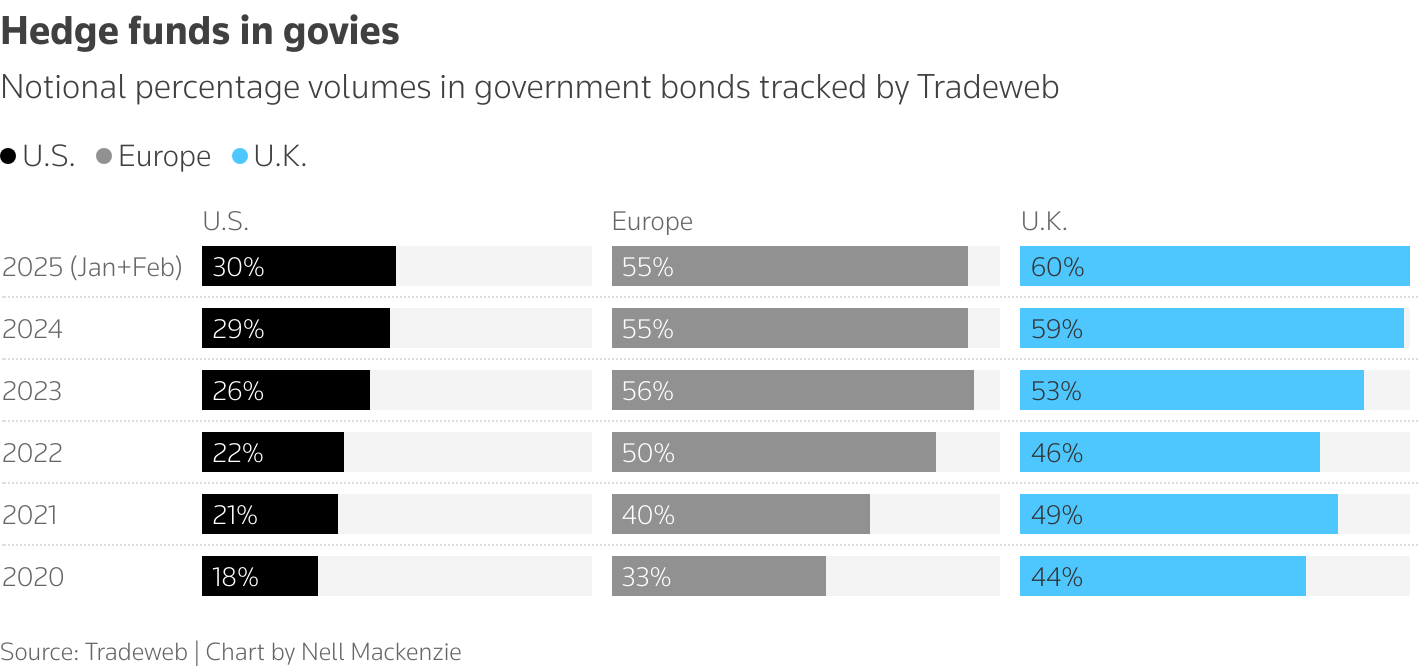
\includegraphics[width=225mm]{../Figures/tradeweb.png}
  \FigNote{Hedge fund share of trading volume in government bonds tracked by Tradeweb.}
\end{minipage}\hfill
\begin{minipage}[c]{370mm}\fBody
\begin{itemize}
  \item Their share of trading volume keeps rising since 2020: in Europe from a third to \textbf{more than half} of volumes.
  \item They finance sovereign positions in the \textbf{repo market}, so leverage ties their funding to the value of the collateral.
  \item Granular evidence on how this footprint affects price formation outside of crises is scarce.
\end{itemize}
\end{minipage}

\vspace{8mm}
\begin{minipage}[t]{302mm}
\begin{tcolorbox}[colback=paleg,colframe=grn,boxrule=1.4pt,arc=3mm,left=7mm,right=7mm,top=3.5mm,bottom=3.5mm]
  \centering{\fHead\bfseries\color{grn}Decrease sensitivity\par}\vspace{2mm}
  {\fBody Arbitrage corrects mispricings.\\Prices are pushed \textit{toward} fundamentals.\par}\vspace{2mm}
  {\fTiny\color{midgrey}Gromb and Vayanos (2002), Cao et al.\ (2018)\par}
\end{tcolorbox}
\end{minipage}\hfill
\begin{minipage}[t]{302mm}
\begin{tcolorbox}[colback=paler,colframe=rust,boxrule=1.4pt,arc=3mm,left=7mm,right=7mm,top=3.5mm,bottom=3.5mm]
  \centering{\fHead\bfseries\color{rust}Increase sensitivity\par}\vspace{2mm}
  {\fBody Leverage and funding fragility force trades.\\Prices are pushed \textit{away} from fundamentals.\par}\vspace{2mm}
  {\fTiny\color{midgrey}Shleifer and Vishny (1997), Brunnermeier and Pedersen (2009)\par}
\end{tcolorbox}
\end{minipage}

\Message{Research question: does the leveraged positioning of hedge funds amplify sovereign bond yield sensitivity to shocks --- and under what conditions?}

% ============================== DATA ==============================
\Section{Data and empirical design}

\begin{minipage}[t]{200mm}
  {\fHead\bfseries\color{navy}Hedge fund repo positions\par}\vspace{1.5mm}
  {\fSmall\color{midgrey}ECB SFTDS\par}\vspace{2mm}
  {\fBody Transaction-level euro area repo data. German and Italian sovereigns, Jan 2021 -- Nov 2025. 152 identified offshore hedge funds. Repo $=$ long, reverse repo $=$ short.\par}
\end{minipage}\hfill
\begin{minipage}[t]{195mm}
  {\fHead\bfseries\color{navy}Bond characteristics\par}\vspace{1.5mm}
  {\fSmall\color{midgrey}Bloomberg\par}\vspace{2mm}
  {\fBody Daily yields, duration, bid-ask spread, amount issued, and cheapest-to-deliver status for each individual bond.\par}
\end{minipage}\hfill
\begin{minipage}[t]{200mm}
  {\fHead\bfseries\color{navy}Exogenous shocks\par}\vspace{1.5mm}
  {\fSmall\color{midgrey}EA-MPD (Altavilla et al.\ 2019)\par}\vspace{2mm}
  {\fBody Intraday 2-year OIS change in the ECB event window. The same shock hits every bond: identification comes from cross-sectional differences in positioning.\par}
\end{minipage}

\vspace{8mm}
\begin{tcolorbox}[colback=pale,colframe=pale,arc=3mm,left=9mm,right=9mm,top=6mm,bottom=6mm]
  \centering\fBody
  $\Delta y_{i,t} \;=\; {\color{rust}\beta_1\,(\mathrm{HF}_{i,t-1} \times \mathrm{Shock}_{t})} \;+\; \beta_2\, \mathrm{HF}_{i,t-1} \;+\; \beta_3\, \mathrm{Shock}_{t} \;+\; \gamma\, \mathbf{X}_{i,t-1} \;+\; \theta_{k} \;+\; \varepsilon_{i,t}$
  \par\vspace{3mm}
  {\fSmall ${\color{rust}\beta_1}$ is the \textbf{additional} yield sensitivity to the shock when hedge funds are positioned in a bond, measured by a presence dummy or by intensity (five-day net position / amount outstanding).\par}
\end{tcolorbox}

\vspace{7mm}
{\fBody\textbf{\color{navy}Identification.} Hedge funds select liquid, large, longer-duration and cheapest-to-deliver bonds. Therefore: duration\,$\times$\,country\,$\times$\,date fixed effects compare similar bonds of the same issuer on the same day; a matched design pairs each hedge fund bond with its closest twin; a dealer-level panel shows the trigger is not dealer behavior.\par}

\vspace{7mm}
\begin{center}
\begin{tabular}{c c c c c}
  {\fStat\bfseries\color{navy}152} & {\fStat\bfseries\color{navy}477{,}001} & {\fStat\bfseries\color{navy}38} & {\fStat\bfseries\color{navy}53\%} & {\fStat\bfseries\color{navy}3\%}\\[2.5mm]
  {\fSmall hedge funds} & {\fSmall bond-days} & {\fSmall ECB announcements} & {\fSmall of bond-days with HF activity} & {\fSmall of an issue held when active}\\
\end{tabular}
\end{center}

% ============================ MECHANISM ============================
\Section{How leveraged positioning amplifies yields}

{\fBody\textbf{Starting point} (Adrian and Shin, 2014): leveraged intermediaries manage their balance sheet against the risk environment --- the same rule produces opposite position adjustments depending on the sign of the shock.\par}
\vspace{6mm}

\begin{center}

\begin{tikzpicture}[box/.style={draw=navy,line width=1.3pt,rounded corners=3mm,align=center,inner xsep=7mm,inner ysep=4mm}]
  \node[box,draw=rust,fill=paler] (con)
    {\fHead\bfseries\color{rust}Constraining\\[1mm]\fBody\color{ink} price moves \textit{against} the position\\ capital buffer erodes $\rightarrow$ fund \textbf{reduces} exposure};
  \node[box,fill=pale,right=16mm of con] (top) {\fHead\bfseries\color{navy} Shock meets a pre-determined\\[1mm]\fHead\bfseries\color{navy} leveraged position};
  \node[box,draw=grn,fill=paleg,right=16mm of top] (rel)
    {\fHead\bfseries\color{grn}Relaxing\\[1mm]\fBody\color{ink} price moves \textit{in favor}\\ constraint loosens $\rightarrow$ fund \textbf{expands} exposure};
  \draw[-{Latex[length=5mm]},line width=1.5pt,navy] (top.west) -- (con.east);
  \draw[-{Latex[length=5mm]},line width=1.5pt,navy] (top.east) -- (rel.west);
\end{tikzpicture}
\end{center}

\vspace{5mm}
{\fBody\textbf{\color{navy}A numerical example} (effective margin 2\%, duration 7y, sector holds 3\% of the issue):\quad 6 bp surprise $\rightarrow$ price $-0.42\%$ $\rightarrow$ capital buffer $\color{rust}\mathbf{-21\%}$ $\rightarrow$ trading pressure $0.63\%$ of the issue $\rightarrow$ $\color{rust}\mathbf{+3.15}$ \textbf{\color{rust}bp} extra yield move.\par}

\Message{In both states the resulting trading pushes yields further in the direction of the initial shock.}

% ============================ FINDING 1 ============================
\Section{Finding 1: Hedge funds increase the volatility of bond yields on shock days}

\begin{minipage}[c]{240mm}
  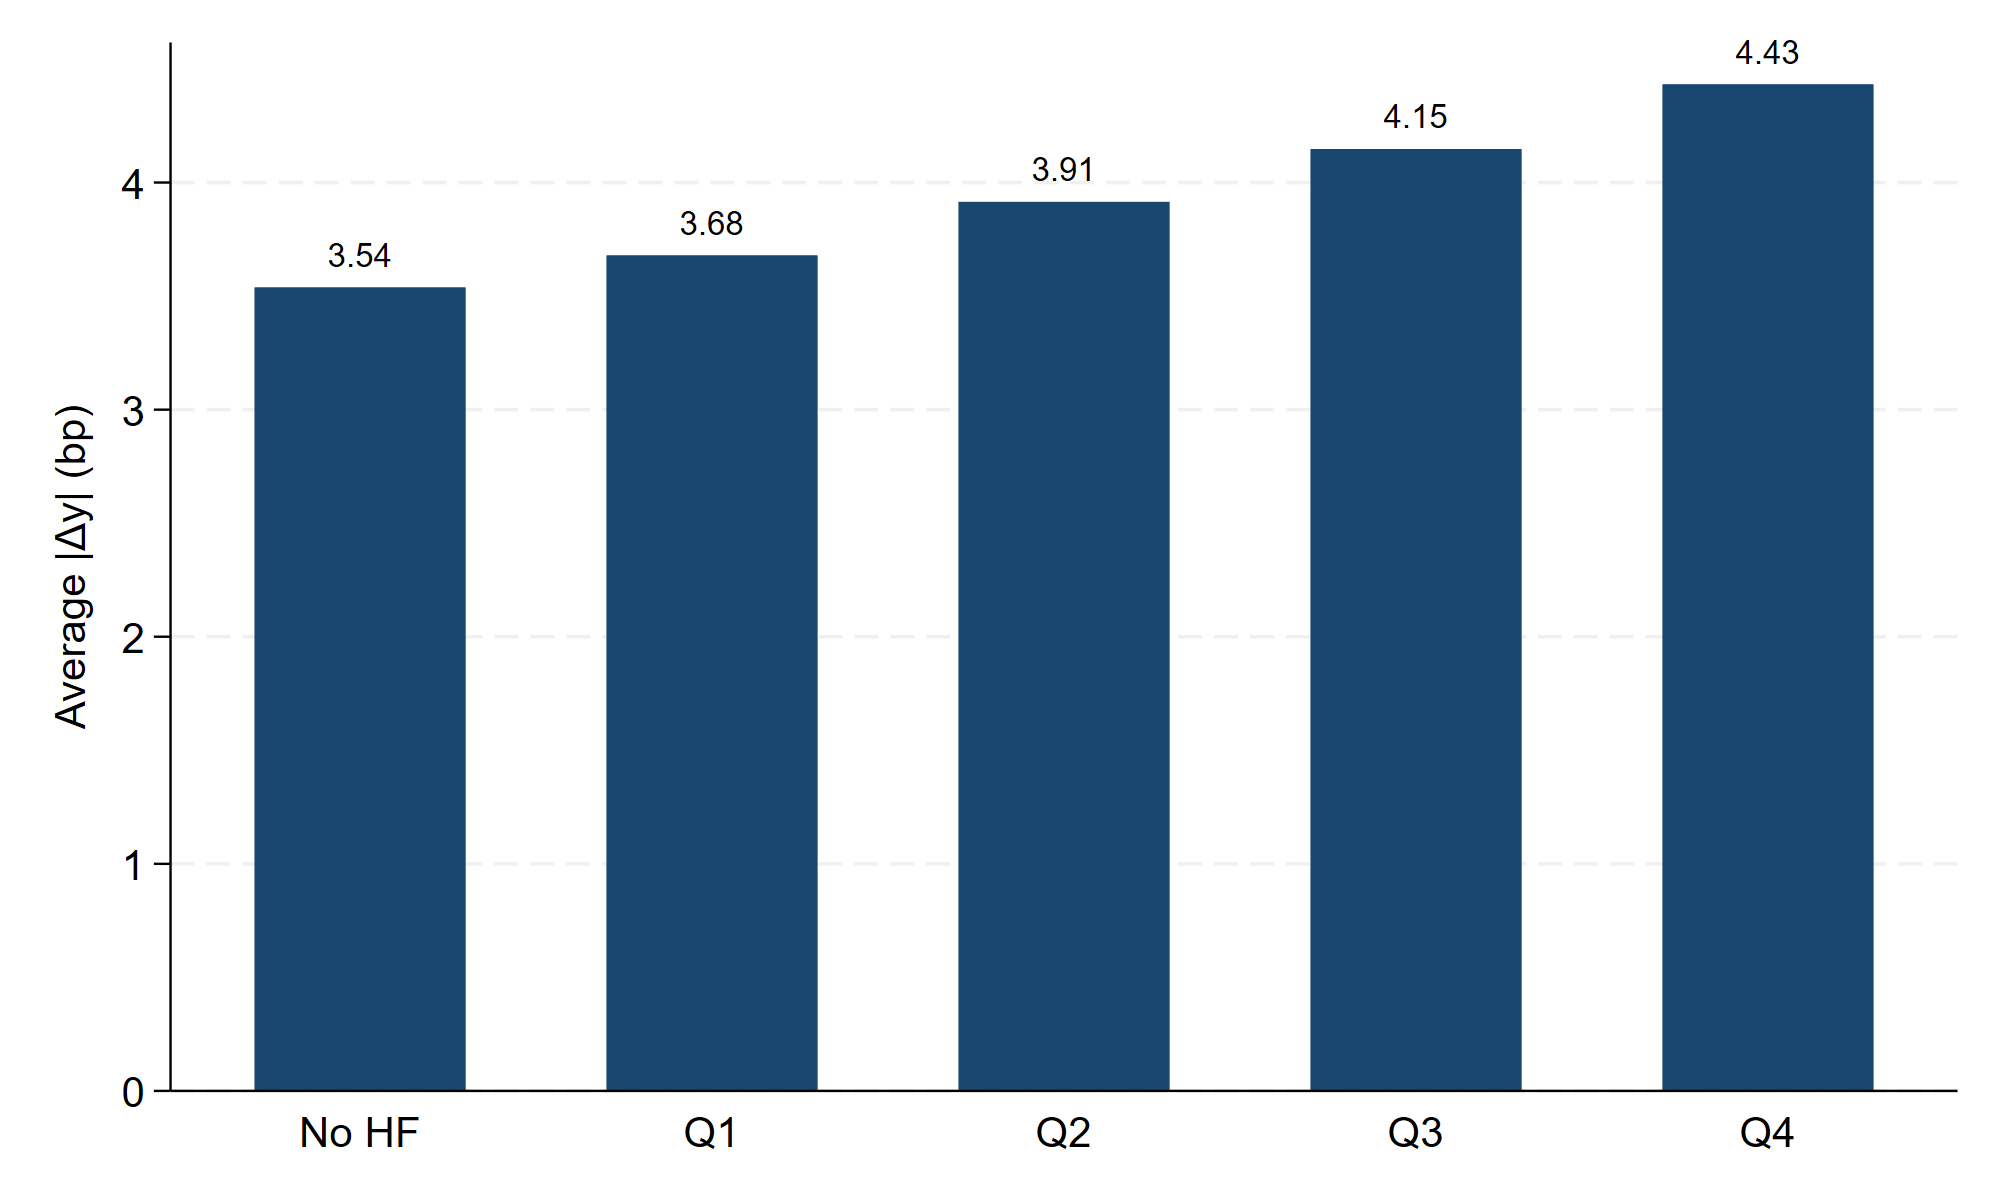
\includegraphics[width=240mm]{../Figures/intensity_volatility_bars.png}
  \FigNote{Average $|\Delta$yield$|$ (bp) on non-shock days by quartile of hedge fund intensity, next to bonds without hedge funds.}
\end{minipage}\hfill
\begin{minipage}[c]{325mm}
  {\fBody Hedge funds do select structurally more volatile bonds. But among \textbf{comparable bonds} (duration $\times$ country $\times$ date cells) the level differential disappears, while the interaction with the shock survives:\par}
  \vspace{5mm}
  \fBody\centering
  \begin{tabular}{l c c}
    \toprule
    $|\Delta \text{yield}|$ (bp) & Raw & Comparable bonds\\
    \midrule
    \textbf{HF involved $\times$ $|$Shock$|$} & \textbf{0.240}$^{***}$ & \textbf{0.246}$^{***}$\\
    HF involved (level) & 0.459$^{***}$ & $-$0.098\\
    \bottomrule
  \end{tabular}
\end{minipage}

\Message{The excess volatility is shock-conditional --- what changes is how yields react to shocks.}

% ============================ FINDING 2 ============================
\Section{Finding 2: Hedge fund trading raises the sensitivity of yields to shocks}

\begin{minipage}[c]{300mm}
  \centering
  
\includegraphics[width=276mm]{figs/shock_reaction_scatterplot.png}
  \FigNote{Binned scatter of daily yield changes against monetary policy surprises, with and without active hedge fund positions.}
\end{minipage}\hfill
\begin{minipage}[c]{300mm}
  \centering
  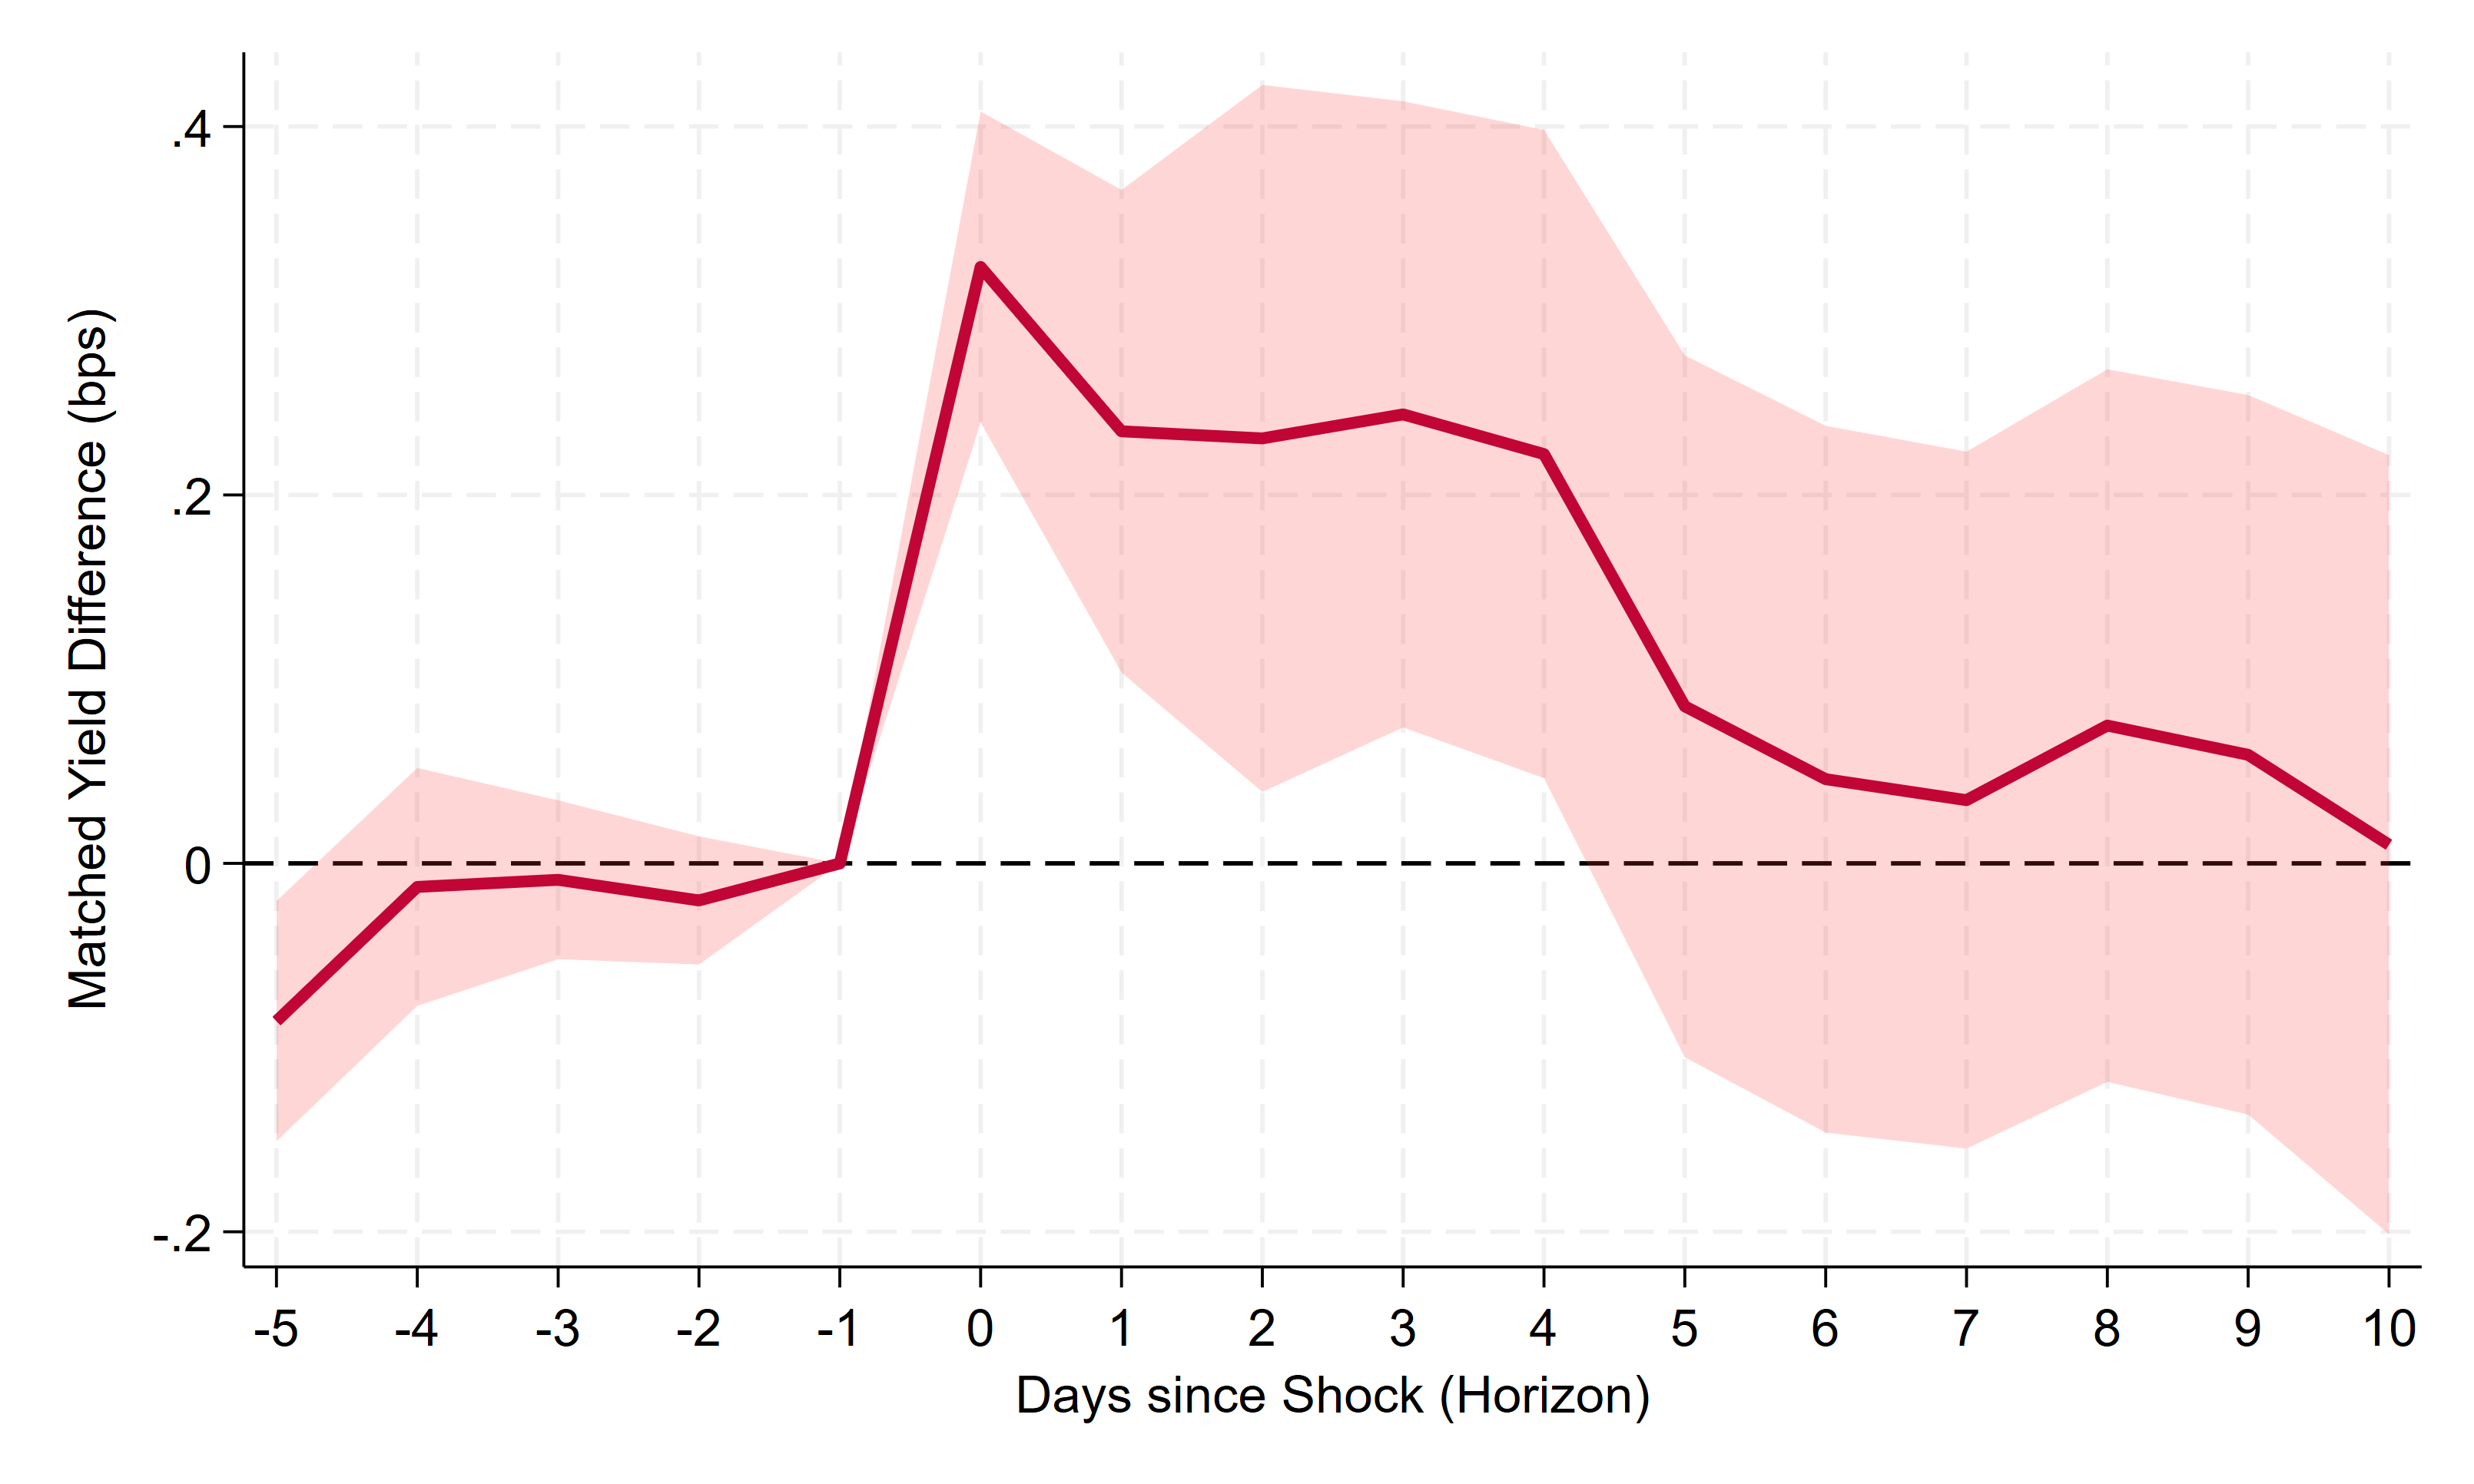
\includegraphics[width=276mm]{../Figures/IR_baseline.png}
  \FigNote{Local projections, matched sample (Jord\`a 2005): flat before the shock, divergence on impact, significant for $\approx$\,4 days, then reversion.}
\end{minipage}

\vspace{6mm}
\begin{minipage}[c]{330mm}
  \fBody\centering
  \begin{tabular}{l c c c}
    \toprule
    $\Delta$ yield (bp) & Baseline & Matched & Intensity\\
    \midrule
    HF involved $\times$ Shock & \textbf{0.291}$^{***}$ & \textbf{0.302}$^{***}$ & \\
    HF intensity $\times$ Shock & & & \textbf{0.164}$^{***}$\\
    HF (level) & $-$0.022 & $-$0.002 & $-$0.011\\
    \bottomrule
  \end{tabular}
  \par\vspace{2mm}
  \FigNote{Duration $\times$ country $\times$ date FE resp.\ matched-pair FE. Within the same bond, a larger position produces a larger reaction --- pure selection cannot explain this.}
\end{minipage}\hfill
\begin{minipage}[c]{270mm}
  \centering
  {\fStat\bfseries\color{rust}$>$\,25\%\par}\vspace{2mm}
  {\fBody of the shock-day yield movement in hedge-fund-traded bonds reflects \textbf{positioning}, not the news itself.\par}
\end{minipage}

\Message{Temporary overshooting that other capital gradually absorbs --- amplification, not price discovery.}

% ============================ FINDING 3 ============================
\Section{Finding 3: The amplification holds whether shocks help or hurt the position}

\begin{minipage}[c]{280mm}
  \fBody
  \centering
  \begin{tabular}{l c c}
    \toprule
    $\Delta$ yield (bp) & {\color{rust}Constraining} & {\color{grn}Relaxing}\\
    \midrule
    HF intensity $\times$ Shock & \textbf{0.140}$^{***}$ & \textbf{0.224}$^{***}$\\
    HF intensity (level) & $-$0.016 & $-$0.009\\
    \bottomrule
  \end{tabular}
  \par\vspace{4mm}
  {\fBody A Wald test cannot distinguish the two regimes ($p=0.16$): the amplification is \textbf{symmetric}.\par}
\end{minipage}\hfill
\begin{minipage}[c]{292mm}
  \centering
  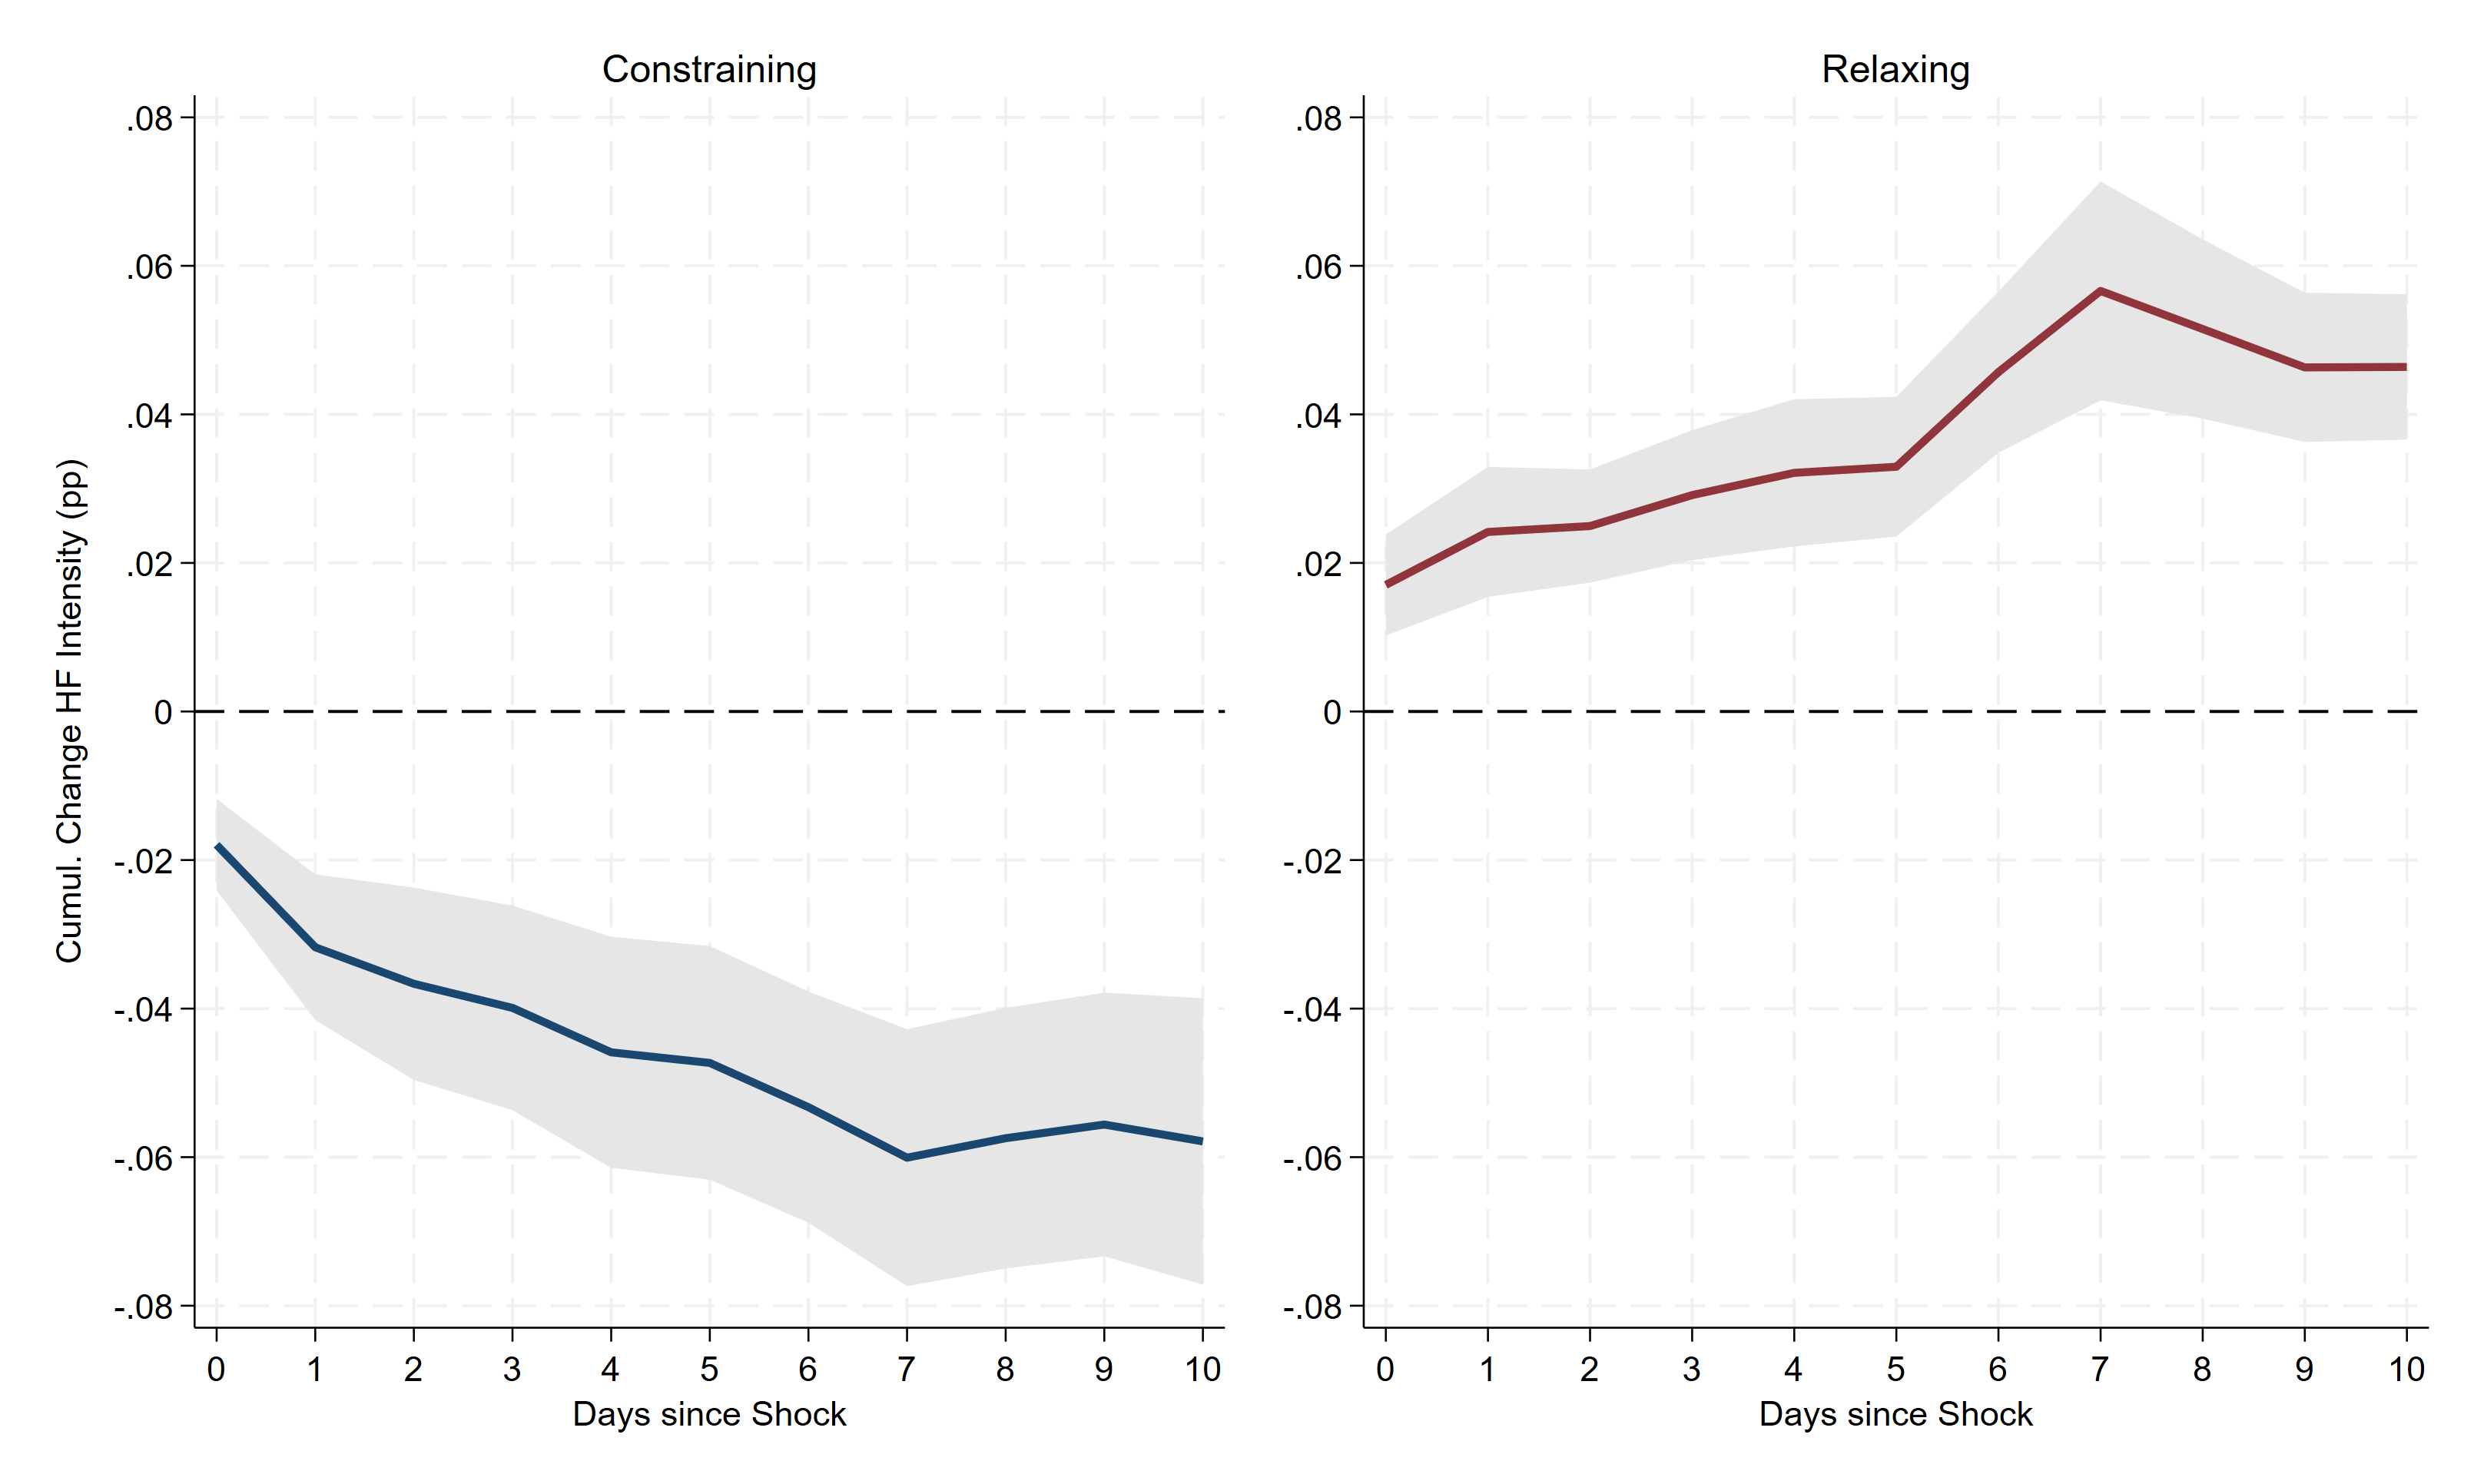
\includegraphics[width=288mm]{../Figures/IR_on_momentum.png}
  \FigNote{Overnight repo positions after the shock: funds contract in the constraining regime and expand in the relaxing regime, as the mechanism predicts.}
\end{minipage}

\Message{Amplification is not only a crisis phenomenon --- it operates whenever shocks meet positions.}

% ============================ FINDING 4 ============================
\Section{Finding 4: The directionality of the book governs the strength}

\begin{minipage}[c]{292mm}
  \centering
  
\includegraphics[width=288mm]{figs/motivation_chart.png}
  \FigNote{Aggregate net repo positions in German (DE) and Italian (IT) sovereigns. Around the hiking cycle: long IT, short DE (hedged book). During it: one-sided short (directional book).}
\end{minipage}\hfill
\begin{minipage}[c]{280mm}
  {\fBody A fund manages one pool of capital against its whole book: a duration-hedged book barely loses capital when rates move, a directional book absorbs the full hit.\par}
  \vspace{4mm}
  \fBody\centering
  \begin{tabular}{l c}
    \toprule
    $\Delta$ yield (bp), rel.\ to no HF & Coefficient\\
    \midrule
    Hedged book $\times$ Shock & 0.098$^{***}$\\
    \textbf{Directional book $\times$ Shock} & \textbf{0.363}$^{***}$\\
    \midrule
    Q1 most hedged $\times$ Shock & 0.057\\
    Q2 $\times$ Shock & 0.137$^{***}$\\
    Q3 $\times$ Shock & 0.361$^{***}$\\
    \textbf{Q4 most directional $\times$ Shock} & \textbf{0.367}$^{***}$\\
    \bottomrule
  \end{tabular}
\end{minipage}

\Message{The amplification rises monotonically with directionality and vanishes when the book is hedged.}

% ========================= CONCLUSION =========================
\Section{Conclusion: what this means for risk monitoring}

\begin{minipage}[t]{300mm}\fBody
\begin{itemize}
  \item Hedge fund positioning amplifies the yield response to shocks: \textbf{more than a quarter} of the shock-day move, reverting within days.
  \item The amplification is \textbf{symmetric} across constraining and relaxing states --- consistent with constant-leverage targeting.
\end{itemize}
\end{minipage}\hfill
\begin{minipage}[t]{300mm}\fBody
\begin{itemize}
  \item Size and presence alone are not sufficient risk metrics, and amplification is \textbf{not confined to stress episodes}.
  \item The \textbf{\color{rust}directionality} of the book is a key risk metric beyond position size.
\end{itemize}
\end{minipage}

\vspace{7mm}
{\fSmall\color{midgrey}\textbf{Robust to:} dealer $\times$ date fixed effects (0.248--0.294$^{***}$, no scaling with dealer CDS stress) $\cdot$ GARCH-standardized yields $\cdot$ sovereign credit (CDS) shocks (0.225$^{***}$) $\cdot$ French and Spanish bonds $\cdot$ placebo with shifted shock dates ($-$0.030, n.s.) $\cdot$ leave-one-out across announcements $\cdot$ randomization inference ($p<0.001$).\par}

\vfill

% ============================= FOOTER =============================
\fullbleed{%
\begin{tcolorbox}[colback=navy,colframe=navy,sharp corners,boxrule=0pt,
    width=710mm,left=50mm,right=50mm,top=10mm,bottom=24mm]
  \color{white}\centering
  {\fSmall Felix Hermes $\cdot$ Goethe University Frankfurt \& European Central Bank $\cdot$ hermes@finance.uni-frankfurt.de\par}
  \vspace{3mm}
  {\fTiny\color{pale}References: Adrian--Shin (2014) $\cdot$ Altavilla et al.\ (2019) $\cdot$ Jord\`a (2005) $\cdot$ Jarocinski--Karadi (2020) $\cdot$ Barth--Kahn (2025) $\cdot$ Kruttli et al.\ (2025) $\cdot$ Gromb--Vayanos (2002) $\cdot$ Brunnermeier--Pedersen (2009)\par}
  \vspace{3mm}
  {\fTiny\color{pale}This poster should not be reported as representing the views of the European Central Bank (ECB). The views expressed are those of the author and do not necessarily reflect those of the ECB.\par}
\end{tcolorbox}}

\end{document}
